\documentclass{article}
%\usepackage{pdftricks}
%\usepackage{pst-all}
% if you use the following package straight latex running (not via pdflatex), will not work...
%\usepackage{pst-pdf}
%\usepackage{auto-pst-pdf}
%\usepackage[pdftex,
%	colorlinks=true,
%	urlcolor=rltblue, % \href{...}{...} external (URL)
%	filecolor=rltgreen, % \href{...} local file
%	linkcolor=rltred, % \ref{...} and \pageref{...}
%	pdftitle={Untitled},
%	pdfauthor={Your Name},
%	pdfsubject={Just a test},
%	pdfkeywords={test, testing, testable stuff},
%	pdfproducer={pdfLaTeX},
%	pagebackref,
%	pdfpagemode=UseNone,
%	bookmarksopen=true]{hyperref} % needed for sketch
%\definecolor{rltred}{rgb}{0.75,0,0}
%\definecolor{rltgreen}{rgb}{0,0.5,0}
%\definecolor{rltblue}{rgb}{0,0,0.75}
%\usepackage{tikz} % for sketch with tikz
%\usepackage{amsmath,color,thumbpdf,html,hyperref}
%\usepackage{pst-barcode,pstricks-add}

% these are the packages that we actually use
\usepackage{thumbpdf} % for thumbnails
\usepackage{hyperref} % for hyperlinks
\usepackage{color} % for colors
\usepackage{amsmath} % for math
\usepackage{amssymb} % for math symbols
\usepackage{pstricks} % for sketch with pstricks support (default for sketch)

\title{Riddles}
\author{Mark Veltzer}
\date{\today}

\begin{document}

\maketitle

\tableofcontents

\section{Rational points on a circle}

%\subsection{Question}

Could there be a circle on the plane where only one point has rational co-ordinates? A point $p=(x,y)$ has rational co-ordinates iff $x,y\in\mathbb{Q}$. What about a sphere? Are there circles with more than one rational point? Are there circles with infinite rational points? Can you find a circle with exactly $n$ rational points on it for each $n\in\mathbb{N}$?

\subsection{Solution}

Yes, there could. Consider the circle: $(x-r)^2+y^2=r^2$ for some irrational $r$.
$(0,0)$ is a point on this circle and is rational. But from the equation it follows
that: $x^2-2xr+r^2+y^2=r^2$ or $x^2+y^2=2xr$ or $r=(x^2+y^2)/2x$. If there
was a rational solution to this equation where $x\ne0$ then it would follow that
$r$ is rational since it is the result of multiplication, division, addition and subtration
of rational numbers and this is a contradiction. This means this equation can only
have rational solutions for $x=0$. If $x=0$ then $r^2+y^2=r^2$ and so $y=0$ and so
$(0,0)$ is the only such solution.

Same solution applies to a sphere: $(x-r)^2+y^2+z^2=r^2$ for some irrational $r$.
In this case: $r=(x^2+y^2+z^2)/2x$. Which means that for $x\ne0$ any rational soultion would imply a rational $r$.
$(0,0,0)$ is therefor the only rational solution.

Yes, there are circles with more than one rational point. Take $x^2+y^2=2$ which is the circle whose
center is at $(0,0)$ and whose radius is $\sqrt{2}$. The points $(1,1),(-1,1),(1,-1),(-1,-1)$ are four rational
points which are on this circle.

Yes, there are circles with infinite rational points (TODO).

What about for each $n\in\mathbb{N}$? (TODO).

\section{Always lead in election (combinatorics)}

%\subsection{Question}

%id=elections (for out of source references to this riddle)

An election was voted a perfect tie (even number of electors) and was decided by way of putting
all the votes into a hat, mixing them uniformly and counting them one by one. What is the chance
that one of the candidates was leading during the entire counting process?

\subsection{Solution}

The question could be rephrased as how many graphs that go either one step up or one step down (lets call those binary graphs) do not go down below zero out of the set of all graphs that go from zero to zero. At first lets note that in the following solution $n$ is even and so there is no problem with $n/2$. A first observation is that the set of all graphs going from 0 to 0 in $n$ steps is ${n \choose n/2}$.

Let's try to count the graphs that tip below 0. Every graph that tips below 0 will reach -1 at one or more points. Lets find the first place where the graph reaches -1. From that point on the graph climbs one more than it descends since it finally reaches 0. Lets flip it from that point on - meaning switch every climb with descent and every descent with a climb. Now the graph descends one more than it climbs and since it starts from that point at height -1 then it now reaches a height -2 at $n$ instead of the original 0.

The main proposition is that \emph{every} graph which travels from 0 to -2 correspons with a \emph{1-1 correspondance} to graphs that travel from 0 to 0 and reach -1 at some point (convince yourself
of this).

If this is so then the number of graphs that go from 0 to -2 is ${n \choose n/2+1}$ since we need to
choose points at which the graph will go down and we have $n/2+1$ descends. If so then the number of
graphs that do not reach -1 is:

${n \choose n/2} - {n \choose n/2+1} = \frac{(n)!}{(n/2+1)!(n/2)!} = \frac{1}{n/2+1}{n \choose n/2}$.

And now back to the original question "What is the chance that one of the candidates was leading during the entire counting process?". Lets divide the latter result with the former and get:

$\frac{1}{n/2+1}{n \choose n/2} / {n \choose n/2} = \frac{1}{n/2+1}$

The result is all about \htmladdnormallink{Catalan numbers}{http://en.wikipedia.org/wiki/Catalan_number}
and \htmladdnormallink{Bertrand's ballot theorem}{http://en.wikipedia.org/wiki/Bertrand\%27s_ballot_theorem}.

\section{Four Coke bottles on a table}

Arrange four Coke bottles on a table so that the distances between each pair of caps will be the same. Assume that
you can make a Coke bottle stand on it's head (this is a pretty strong hint!, maybe I should remove it ?!?). The length
or height of each bottle is ${h}$.

\subsection{Solution}

There are two solutions:

The first solution is to put the bottles in a square where the side of the square is the length of the bottle. Bottles
next to each other will stand \emph{in reverse} (if the first is on it's head the the second will stand straight).

\begin{center}
% Sketch output, version 0.3 (build 7d, Wed May 2 06:36:52 2012)
% Output language: PGF/TikZ,LaTeX
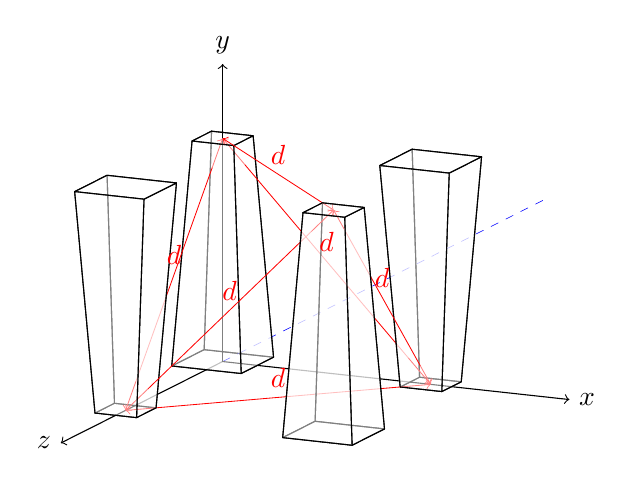
\begin{tikzpicture}[line join=round]
\draw[arrows=-](-2.055,-1.034)--(-2.261,-1.138);
\filldraw[fill opacity=0.5,fill=white](-2.29,-.883)--(-2.701,-1.09)--(-1.82,-1.186)--(-1.409,-.979)--cycle;
\draw[line width=.2pt,draw=blue,dashed](-1.85,-.931)--(2.055,1.034);
\filldraw[fill opacity=0.5,fill=white](-1.409,-.979)--(-2.29,-.883)--(-2.196,1.891)--(-1.668,1.833)--cycle;
\filldraw[fill opacity=0.5,fill=white](-2.29,-.883)--(-2.701,-1.09)--(-2.443,1.767)--(-2.196,1.891)--cycle;
\draw[line width=.2pt,draw=blue,dashed](-2.055,-1.034)--(-1.85,-.931);
\draw[arrows=-](-2.055,-1.034)--(-1.615,-1.083);
\draw[line width=.3pt,arrows=<-,draw=red](-2.055,1.8)--(-1.772,1.465);
\filldraw[fill opacity=0.5,fill=white](-1.82,-1.186)--(-1.409,-.979)--(-1.668,1.833)--(-1.914,1.709)--cycle;
\draw[arrows=-](-2.055,-1.034)--(-2.055,1.8);
\filldraw[fill opacity=0.5,fill=white](.975,-1.291)--(.728,-1.415)--(.2,-1.357)--(.446,-1.233)--cycle;
\draw[arrows=-](-1.615,-1.083)--(.323,-1.295);
\draw[line width=.3pt,arrows=->,draw=red](-2.187,1.43)--(-2.055,1.8);
\filldraw[fill opacity=0.5,fill=white](-2.701,-1.09)--(-1.82,-1.186)--(-1.914,1.709)--(-2.443,1.767)--cycle;
\filldraw[fill opacity=0.5,fill=white](-2.196,1.891)--(-2.443,1.767)--(-1.914,1.709)--(-1.668,1.833)--cycle;
\draw[arrows=-](-2.261,-1.138)--(-3.165,-1.593);
\draw[arrows=->](-2.055,1.8)--(-2.055,2.745);
\draw[line width=.3pt,arrows=<-,draw=red](-2.055,1.8)--(-1.914,1.709);
\draw[line width=.3pt,arrows=-,draw=red](-1.772,1.465)--(.304,-.989);
\filldraw[fill opacity=0.5,fill=white](-.059,1.455)--(.352,1.662)--(.446,-1.233)--(.2,-1.357)--cycle;
\filldraw[fill opacity=0.5,fill=white](.352,1.662)--(1.233,1.566)--(.975,-1.291)--(.446,-1.233)--cycle;
\draw[line width=.3pt,arrows=-,draw=red](-3.156,-1.285)--(-2.187,1.43);
\draw[line width=.3pt,arrows=-,draw=red](-1.914,1.709)--(-.787,.981);
\draw[arrows=-](.323,-1.295)--(.851,-1.353);
\filldraw[fill opacity=0.5,fill=white](1.233,1.566)--(.822,1.359)--(.728,-1.415)--(.975,-1.291)--cycle;
\draw[line width=.3pt,arrows=->,draw=red](.304,-.989)--(.587,-1.324);
\draw[line width=.3pt,arrows=<-,draw=red](.587,-1.324)--(.2,-1.357);
\draw[line width=.3pt,arrows=<-,draw=red](.587,-1.324)--(.455,-1.087);
\filldraw[fill opacity=0.5,fill=white](1.233,1.566)--(.822,1.359)--(-.059,1.455)--(.352,1.662)--cycle;
\draw[arrows=->](.851,-1.353)--(2.349,-1.517);
\filldraw[fill opacity=0.5,fill=white](.822,1.359)--(-.059,1.455)--(.2,-1.357)--(.728,-1.415)--cycle;
\filldraw[fill opacity=0.5,fill=white](-2.901,-1.622)--(-3.148,-1.746)--(-3.676,-1.688)--(-3.429,-1.564)--cycle;
\draw[line width=.3pt,arrows=-,draw=red](.2,-1.357)--(-2.901,-1.622);
\draw[line width=.3pt,arrows=-,draw=red](.455,-1.087)--(-.514,.652);
\filldraw[fill opacity=0.5,fill=white](-3.523,1.331)--(-2.642,1.234)--(-2.901,-1.622)--(-3.429,-1.564)--cycle;
\filldraw[fill opacity=0.5,fill=white](-3.934,1.124)--(-3.523,1.331)--(-3.429,-1.564)--(-3.676,-1.688)--cycle;
\draw[arrows=-](-3.165,-1.593)--(-3.412,-1.717);
\draw[line width=.3pt,arrows=<-,draw=red](-3.288,-1.655)--(-3.156,-1.285);
\draw[line width=.3pt,arrows=->,draw=red](-2.901,-1.622)--(-3.288,-1.655);
\draw[line width=.3pt,arrows=->,draw=red](-3.005,-1.383)--(-3.288,-1.655);
\filldraw[fill opacity=0.5,fill=white](-2.642,1.234)--(-3.054,1.028)--(-3.148,-1.746)--(-2.901,-1.622)--cycle;
\filldraw[fill opacity=0.5,fill=white](-2.642,1.234)--(-3.054,1.028)--(-3.934,1.124)--(-3.523,1.331)--cycle;
\filldraw[fill opacity=0.5,fill=white](-3.054,1.028)--(-3.934,1.124)--(-3.676,-1.688)--(-3.148,-1.746)--cycle;
\filldraw[fill opacity=0.5,fill=white](0,-1.89)--(-.881,-1.793)--(-.787,.981)--(-.258,.923)--cycle;
\draw[line width=.3pt,arrows=-,draw=red](-.929,.617)--(-3.005,-1.383);
\draw[arrows=->](-3.412,-1.717)--(-4.111,-2.069);
\filldraw[fill opacity=0.5,fill=white](-.881,-1.793)--(-1.292,-2)--(-1.034,.857)--(-.787,.981)--cycle;
\filldraw[fill opacity=0.5,fill=white](-.881,-1.793)--(-1.292,-2)--(-.411,-2.097)--(0,-1.89)--cycle;
\filldraw[fill opacity=0.5,fill=white](-.411,-2.097)--(0,-1.89)--(-.258,.923)--(-.505,.799)--cycle;
\draw[line width=.3pt,arrows=->,draw=red](-.514,.652)--(-.646,.89);
\draw[line width=.3pt,arrows=<-,draw=red](-.646,.89)--(-.929,.617);
\filldraw[fill opacity=0.5,fill=white](-1.292,-2)--(-.411,-2.097)--(-.505,.799)--(-1.034,.857)--cycle;
\draw[line width=.3pt,arrows=->,draw=red](-.787,.981)--(-.646,.89);
\filldraw[fill opacity=0.5,fill=white](-.787,.981)--(-1.034,.857)--(-.505,.799)--(-.258,.923)--cycle;
\node[right] at (2.349,-1.517) {$x$};\node[above] at (-2.055,2.745) {$y$};\node[left] at (-4.111,-2.069) {$z$};\node[above,color=red] at (-1.351,1.345) {$d$};\node[above,color=red] at (-1.351,-1.49) {$d$};\node[above,color=red] at (-.734,.238) {$d$};\node[above,color=red] at (-.029,-.217) {$d$};\node[above,color=red] at (-1.967,-.383) {$d$};\node[above,color=red] at (-2.672,.072) {$d$};\end{tikzpicture}% End sketch output

\end{center}

The shape created by the bottle caps is, ofcourse, a perfect triangular pyramid with a side of length $d=\sqrt{2h^2}$.

The second solution is to put three bottles on the vertices of an equilateral triangle standing one way. The fourth will be placed
in the middle of the triangle and will be standing reversed to the others. The problem here is to calculate the side of the triangle.
Lets use the following diagram:

\begin{center}
% Sketch output, version 0.3 (build 7d, Sun Mar 20 14:11:05 2016)
% Output language: PGF/TikZ,LaTeX
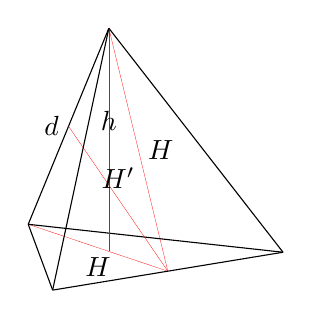
\begin{tikzpicture}[line join=round]
\draw[line width=.1pt,draw=red](-2.055,-1.034)--(-.282,-1.63);
\draw(-2.055,-1.034)--(-1.745,-1.87);
\draw(-1.031,1.456)--(-2.055,-1.034);
\draw(-2.055,-1.034)--(1.181,-1.389);
\draw[line width=.1pt,draw=red](-.282,-1.63)--(-1.543,.211);
\draw[line width=.1pt,draw=red](-1.031,1.456)--(-1.031,-1.378);
\draw(1.181,-1.389)--(-1.031,1.456);
\draw(1.181,-1.389)--(-1.745,-1.87);
\draw(-1.745,-1.87)--(-1.031,1.456);
\draw[line width=.1pt,draw=red](-1.031,1.456)--(-.282,-1.63);
\node[below] at (-1.169,-1.332) {$H$};\node[right] at (-.657,-.087) {$H$};\node[above] at (-1.031,.039) {$h$};\node[above] at (-.913,-.709) {$H'$};\node[left] at (-1.543,.211) {$d$};\end{tikzpicture}% End sketch output

\end{center}

What we are trying to find is $d$ as a function of $h$. Since $H$, $d/2$ and $d$ create a right angeled triangle, it follows
that $H^2+(d/2)^2=d^2$ and so $H=\sqrt{3}/2d$. Since the size of the inner triangle could be computed two ways then $hH=dH'$ and
since $H'=\sqrt{H^2-(d/2)^2}$ it follows after some math that $d=\sqrt{3/2}h$ which makes $d$ about $1.224h$.

The solution built on this analysis will look like this:

\begin{center}
% Sketch output, version 0.3 (build 7d, Wed May 2 06:36:52 2012)
% Output language: PGF/TikZ,LaTeX
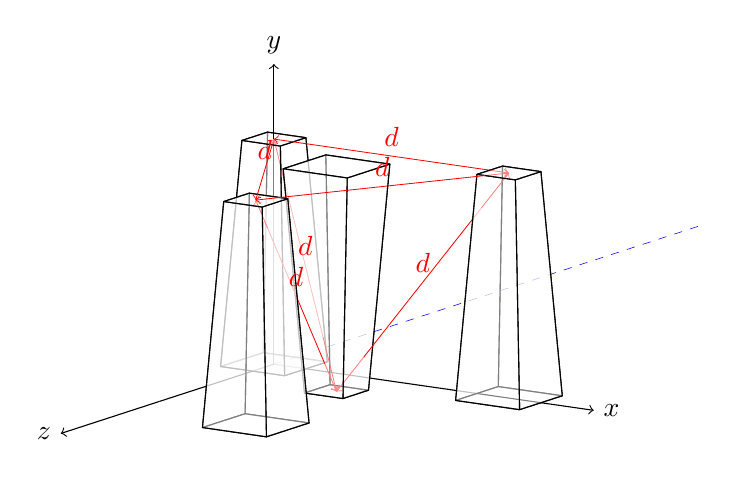
\begin{tikzpicture}[line join=round]
\draw[line width=.2pt,draw=blue,dashed](-2.437,-.792)--(2.708,.88);
\filldraw[fill opacity=0.5,fill=white](-2.031,-.85)--(-2.843,-.733)--(-2.789,2.067)--(-2.302,1.997)--cycle;
\filldraw[fill opacity=0.5,fill=white](-2.843,-.733)--(-3.385,-.909)--(-3.114,1.962)--(-2.789,2.067)--cycle;
\draw[line width=.2pt,draw=blue,dashed](-2.708,-.88)--(-2.437,-.792);
\draw[arrows=-](-2.708,-.88)--(-2.302,-.938);
\filldraw[fill opacity=0.5,fill=white](-2.843,-.733)--(-3.385,-.909)--(-2.572,-1.026)--(-2.031,-.85)--cycle;
\draw[line width=.3pt,arrows=->,draw=red](-2.536,1.288)--(-2.708,1.979);
\filldraw[fill opacity=0.5,fill=white](-2.572,-1.026)--(-2.031,-.85)--(-2.302,1.997)--(-2.626,1.891)--cycle;
\draw[arrows=-](-2.708,-.88)--(-2.978,-.968);
\draw[arrows=-](-2.708,-.88)--(-2.708,1.979);
\filldraw[fill opacity=0.5,fill=white](-3.385,-.909)--(-2.572,-1.026)--(-2.626,1.891)--(-3.114,1.962)--cycle;
\draw[line width=.3pt,arrows=<-,draw=red](-2.708,1.979)--(-2.729,1.906);
\filldraw[fill opacity=0.5,fill=white](-2.789,2.067)--(-3.114,1.962)--(-2.626,1.891)--(-2.302,1.997)--cycle;
\draw[arrows=-](-2.302,-.938)--(-1.659,-1.031);
\draw[arrows=-](-2.978,-.968)--(-4.16,-1.352);
\draw[arrows=->](-2.708,1.979)--(-2.708,2.933);
\draw[line width=.3pt,arrows=<-,draw=red](-2.708,1.979)--(-2.464,1.944);
\draw[arrows=-](-1.659,-1.031)--(-1.172,-1.102);
\draw[line width=.3pt,arrows=-,draw=red](-2.464,1.944)--(.033,1.584);
\draw[line width=.3pt,arrows=-,draw=red](-2.084,-.536)--(-2.536,1.288);
\draw[line width=.3pt,arrows=-,draw=red](-2.729,1.906)--(-2.917,1.277);
\draw[arrows=-](-1.172,-1.102)--(-.129,-1.252);
\filldraw[fill opacity=0.5,fill=white](-2.59,1.602)--(-2.048,1.778)--(-1.994,-1.14)--(-2.319,-1.246)--cycle;
\filldraw[fill opacity=0.5,fill=white](-1.507,-1.21)--(-1.831,-1.316)--(-2.319,-1.246)--(-1.994,-1.14)--cycle;
\filldraw[fill opacity=0.5,fill=white](-2.048,1.778)--(-1.236,1.661)--(-1.507,-1.21)--(-1.994,-1.14)--cycle;
\draw[line width=.3pt,arrows=-,draw=red](-.072,1.106)--(-.637,.389);
\filldraw[fill opacity=0.5,fill=white](.142,-1.164)--(-.4,-1.34)--(-.129,1.531)--(.196,1.636)--cycle;
\filldraw[fill opacity=0.5,fill=white](.954,-1.281)--(.142,-1.164)--(.196,1.636)--(.683,1.566)--cycle;
\filldraw[fill opacity=0.5,fill=white](.142,-1.164)--(-.4,-1.34)--(.412,-1.457)--(.954,-1.281)--cycle;
\draw[line width=.3pt,arrows=<-,draw=red](-1.913,-1.228)--(-2.084,-.536);
\draw[line width=.3pt,arrows=->,draw=red](-1.564,-.786)--(-1.913,-1.228);
\filldraw[fill opacity=0.5,fill=white](-1.236,1.661)--(-1.777,1.485)--(-1.831,-1.316)--(-1.507,-1.21)--cycle;
\filldraw[fill opacity=0.5,fill=white](-1.236,1.661)--(-1.777,1.485)--(-2.59,1.602)--(-2.048,1.778)--cycle;
\draw[line width=.3pt,arrows=->,draw=red](-2.062,-.874)--(-1.913,-1.228);
\filldraw[fill opacity=0.5,fill=white](-1.777,1.485)--(-2.59,1.602)--(-2.319,-1.246)--(-1.831,-1.316)--cycle;
\draw[arrows=-](-.129,-1.252)--(.683,-1.369);
\draw[line width=.3pt,arrows=-,draw=red](-.999,-.069)--(-1.564,-.786);
\filldraw[fill opacity=0.5,fill=white](.412,-1.457)--(.954,-1.281)--(.683,1.566)--(.358,1.461)--cycle;
\draw[line width=.3pt,arrows=-,draw=red](-2.789,.85)--(-2.062,-.874);
\draw[line width=.3pt,arrows=-,draw=red](-.637,.389)--(-.999,-.069);
\draw[line width=.3pt,arrows=<-,draw=red](.277,1.548)--(-.072,1.106);
\filldraw[fill opacity=0.5,fill=white](-.4,-1.34)--(.412,-1.457)--(.358,1.461)--(-.129,1.531)--cycle;
\draw[arrows=->](-4.16,-1.352)--(-5.415,-1.76);
\draw[line width=.3pt,arrows=->,draw=red](.033,1.584)--(.277,1.548);
\draw[line width=.3pt,arrows=<-,draw=red](.277,1.548)--(-.026,1.516);
\filldraw[fill opacity=0.5,fill=white](.196,1.636)--(-.129,1.531)--(.358,1.461)--(.683,1.566)--cycle;
\draw[arrows=->](.683,-1.369)--(1.354,-1.466);
\draw[line width=.3pt,arrows=-,draw=red](-.026,1.516)--(-.248,1.492);
\draw[line width=.3pt,arrows=-,draw=red](-.248,1.492)--(-1.157,1.395);
\filldraw[fill opacity=0.5,fill=white](-2.262,-1.626)--(-3.074,-1.509)--(-3.02,1.292)--(-2.532,1.222)--cycle;
\filldraw[fill opacity=0.5,fill=white](-3.074,-1.509)--(-3.615,-1.684)--(-3.345,1.186)--(-3.02,1.292)--cycle;
\filldraw[fill opacity=0.5,fill=white](-3.074,-1.509)--(-3.615,-1.684)--(-2.803,-1.802)--(-2.262,-1.626)--cycle;
\draw[line width=.3pt,arrows=-,draw=red](-1.157,1.395)--(-2.494,1.252);
\draw[line width=.3pt,arrows=<-,draw=red](-2.939,1.204)--(-2.789,.85);
\filldraw[fill opacity=0.5,fill=white](-2.803,-1.802)--(-2.262,-1.626)--(-2.532,1.222)--(-2.857,1.116)--cycle;
\filldraw[fill opacity=0.5,fill=white](-3.615,-1.684)--(-2.803,-1.802)--(-2.857,1.116)--(-3.345,1.186)--cycle;
\filldraw[fill opacity=0.5,fill=white](-3.02,1.292)--(-3.345,1.186)--(-2.857,1.116)--(-2.532,1.222)--cycle;
\draw[line width=.3pt,arrows=->,draw=red](-2.917,1.277)--(-2.939,1.204);
\draw[line width=.3pt,arrows=-,draw=red](-2.494,1.252)--(-2.635,1.237);
\draw[line width=.3pt,arrows=->,draw=red](-2.635,1.237)--(-2.939,1.204);
\node[right] at (1.354,-1.466) {$x$};\node[above] at (-2.708,2.933) {$y$};\node[left] at (-5.415,-1.76) {$z$};\node[above,color=red] at (-2.823,1.592) {$d$};\node[above,color=red] at (-.818,.16) {$d$};\node[above,color=red] at (-1.215,1.764) {$d$};\node[above,color=red] at (-1.331,1.376) {$d$};\node[above,color=red] at (-2.426,-.012) {$d$};\node[above,color=red] at (-2.31,.376) {$d$};\end{tikzpicture}% End sketch output

\end{center}

As is evident the key to solving this question is the perfect triangular pyramid as both solutions are based on it and it is the only
way to put 4 elements in space being spaced equally apart. In theory you could place the bottles at any height and so
infinite solutions to this riddle could be produced by making the side of the perfect pyramid as small or as large as you want. But we are
constrained by the table and so the heights at which the caps are will be either $0$ or $h$. The two solutions above seem to be primary
examples under this constraint. Minor variations on the above two solutions could be produced by making the bottles whose caps are at table
level lay instead of stand on their heads. The first solution is more attractive than the second because it could be performed in practice
without relying on measurement tools in order to place the bottles at the calculated distance from each other as per the second solution.

\label{end}\end{document}
